%%=============================================================================
%% Resultaten
%%=============================================================================

\chapter{Resultaten}
\label{ch:resultaten}

Om de verschillende modellen te testen, worden meerdere scenario’s gehanteerd.
Ten eerste wordt gebruikgemaakt van een testset met tien vragen waarvan de informatie beschikbaar is in de documentatie. Van elk model wordt verwacht dat het op iedere vraag een concreet antwoord geeft. Deze antwoorden worden vervolgens geëvalueerd met behulp van het test framework Ragas, waarbij vier verschillende meetcriteria worden toegepast.
\\[1em]
Het tweede testscenario bestaat uit het stellen van niet-triviale vragen waarvoor de informatie niet beschikbaar is in de documentatie. Dit scenario is vooral bedoeld om te onderzoeken of bepaalde modellen tekenen van hallucinaties vertonen.
\\[1em]
Ten slotte worden enkele triviale vragen gesteld. Hierbij wordt getest of het model in staat is een juiste inschatting te maken door direct te antwoorden, zonder onnodige zoekopdrachten in de vector database.

%TODO aanpassen waar nodig

\section{Evaluatie 1: Documentatiegebaseerde vragen}

De verschillende modellen kregen elk een vragenlijst, waarvan het verwachte antwoord te vinden is in bijlage \ref{vragenlijst}. Daarnaast zijn de antwoorden van elk model terug te vinden in bijlage %TODO.
\\[1em]
Wanneer in de categorie Faithfulness een waarde van 0,000 aanwezig is, betekent dit dat het model ten onrechte heeft besloten de retriever-tool niet te gebruiken.
Op basis van deze tests werden de volgende resultaten vastgesteld:

\subsection{Llama3.1}

\begin{table}[H]
    \centering
    \begin{tabular}{|l|c|c|c|c|}
        \hline
        \textbf{Vraag} & \textbf{Faithfulness} & \textbf{Response relevancy} & \textbf{Answer correctness} & \textbf{Context recall} \\
        \hline
        Vraag 1 & 1.000 & 0.000 & 0.225 & 0.500 \\
        Vraag 2 & 0.333 & 0.000 & 0.221 & 0.000 \\
        Vraag 3 & 0.385 & 0.000 & 0.223 & 0.500 \\
        Vraag 4 & 0.000 & 0.000 & 0.174 & 1.000 \\
        Vraag 5 & 1.000 & 0.863 & 0.212 & 0.125 \\
        Vraag 6 & 0.667 & 0.920 & 0.477 & 1.000 \\
        Vraag 7 & 0.500 & 0.000 & 0.205 & 1.000 \\
        Vraag 8 & 0.714 & 0.000 & 0.408 & 1.000 \\
        Vraag 9 & 0.500 & 0.932 & 0.391 & 1.000 \\
        Vraag 10 & 0.333 & 0.000 & 0.205 & 1.000 \\
        \hline
    \end{tabular}
    \caption{Resultaten per vraag op de vier meetcriteria van het Llama3.1 model.}
    \label{tab:resultaten_vragen_llama3.1}
\end{table}

\subsection{Llama3.2}

\begin{table}[H]
    \centering
    \begin{tabular}{|l|c|c|c|c|}
        \hline
        \textbf{Vraag} & \textbf{Faithfulness} & \textbf{Response relevancy} & \textbf{Answer correctness} & \textbf{Context recall} \\
        \hline
        Vraag 1  & 0.500 & 0.894 & 0.485 & 0.500 \\
        Vraag 2  & 0.333 & 0.000 & 0.220 & 0.000 \\
        Vraag 3  & 0.800 & 0.000 & 0.219 & 0.500 \\
        Vraag 4  & 0.571 & 0.863 & 0.196 & 0.833 \\
        Vraag 5  & 0.625 & 0.000 & 0.205 & 0.125 \\
        Vraag 6  & 0.857 & 0.000 & 0.194 & 1.000 \\
        Vraag 7  & 0.917 & 0.860 & 0.991 & 1.000 \\
        Vraag 8  & 0.833 & 0.953 & 0.212 & 1.000 \\
        Vraag 9  & 0.429 & 0.883 & 0.631 & 0.375 \\
        Vraag 10 & 0.333 & 0.000 & 0.207 & 1.000 \\
        \hline
    \end{tabular}
    \caption{Resultaten per vraag op de vier meetcriteria van het Llama3.2 model.}
    \label{tab:resultaten_vragen_llama3.2}
\end{table}

\subsection{Qwen2.5}

\begin{table}[H]
    \centering
    \begin{tabular}{|l|c|c|c|c|}
        \hline
        \textbf{Vraag} & \textbf{Faithfulness} & \textbf{Response relevancy} & \textbf{Answer correctness} & \textbf{Context recall} \\
        \hline
        Vraag 1  & 0.750 & 0.000 & 0.485 & 0.500 \\
        Vraag 2  & 0.500 & 0.000 & 0.226 & 0.000 \\
        Vraag 3  & 0.929 & 0.000 & 0.229 & 0.500 \\
        Vraag 4  & 0.000 & 0.000 & 0.174 & 1.000 \\
        Vraag 5  & 0.000 & 0.000 & 0.180 & 0.000 \\
        Vraag 6  & 1.000 & 0.871 & 0.469 & 1.000 \\
        Vraag 7  & 0.000 & 0.000 & 0.176 & 1.000 \\
        Vraag 8  & 0.000 & 0.000 & 0.179 & 0.000 \\
        Vraag 9  & 0.000 & 0.000 & 0.176 & 0.556 \\
        Vraag 10 & 0.667 & 0.000 & 0.216 & 0.000 \\
        \hline
    \end{tabular}
    \caption{Resultaten per vraag op de vier meetcriteria van het Qwen2.5 model.}
    \label{tab:resultaten_vragen_qwen2.5}
\end{table}


\subsection{Qwen3}

\begin{table}[H]
    \centering
    \begin{tabular}{|l|c|c|c|c|}
        \hline
        \textbf{Vraag} & \textbf{Faithfulness} & \textbf{Response relevancy} & \textbf{Answer correctness} & \textbf{Context recall} \\
        \hline
        Vraag 1  & 1.000 & 0.000 & 0.216 & 0.500 \\
        Vraag 2  & 1.000 & 0.000 & 0.224 & 0.000 \\
        Vraag 3  & 1.000 & 0.000 & 0.220 & 0.250 \\
        Vraag 4  & 0.857 & 0.000 & 0.203 & 0.000 \\
        Vraag 5  & 0.636 & 0.867 & 0.211 & 0.125 \\
        Vraag 6  & 0.750 & 0.874 & 0.571 & 1.000 \\
        Vraag 7  & 1.000 & 0.906 & 0.989 & 1.000 \\
        Vraag 8  & 0.556 & 0.000 & 0.411 & 1.000 \\
        Vraag 9  & 1.000 & 0.000 & 0.340 & 0.625 \\
        Vraag 10 & 1.000 & 0.935 & 0.636 & 1.000 \\
        \hline
    \end{tabular}
    \caption{Resultaten per vraag op de vier meetcriteria van het Qwen3 model.}
    \label{tab:resultaten_vragen_qwen3}
\end{table}


\subsection{Samenvatting}

Om de prestaties van de modellen per individuele metric te vergelijken, worden in figuur~\ref{fig:vergelijking_metrics} vier staafdiagrammen weergegeven: Faithfulness, Response relevancy, Answer correctness en Context recall.

\begin{figure}[H]
    \centering
    \begin{subfigure}{0.48\textwidth}
        \centering
        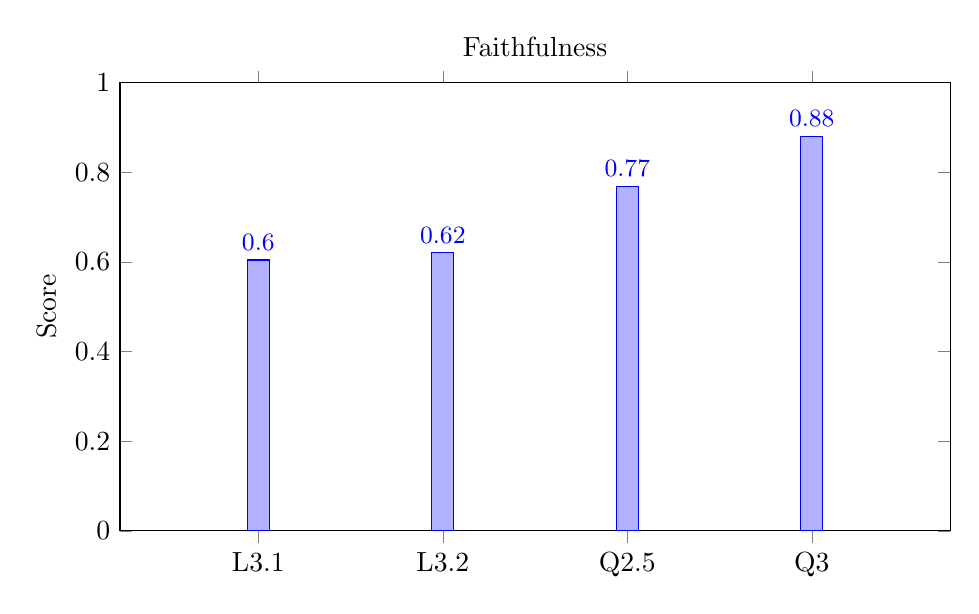
\begin{tikzpicture}
            \begin{axis}[
                ybar,
                ymin=0,
                ymax=1,
                bar width=8pt,
                width=\textwidth,
                height=0.6\textwidth,
                enlarge x limits=0.25,
                ylabel={Score},
                symbolic x coords={L3.1,L3.2,Q2.5,Q3},
                xtick=data,
                nodes near coords,
                nodes near coords align={vertical},
                every node near coord/.append style={font=\small},
                title={Faithfulness}
                ]
                \addplot coordinates {(L3.1,0.604) (L3.2,0.620) (Q2.5, 0.769) (Q3,0.880)};
            \end{axis}
        \end{tikzpicture}
    \end{subfigure}
    \hfill
    \begin{subfigure}{0.48\textwidth}
        \centering
        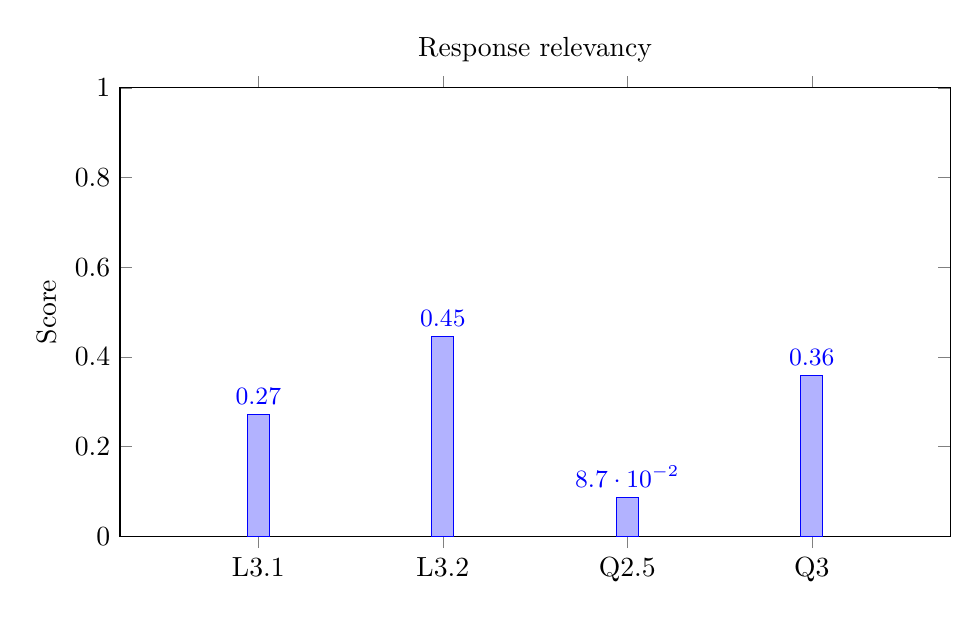
\begin{tikzpicture}
            \begin{axis}[
                ybar,
                ymin=0,
                ymax=1,
                bar width=8pt,
                width=\textwidth,
                height=0.6\textwidth,
                enlarge x limits=0.25,
                ylabel={Score},
                symbolic x coords={L3.1,L3.2,Q2.5,Q3},
                xtick=data,
                nodes near coords,
                nodes near coords align={vertical},
                every node near coord/.append style={font=\small},
                title={Response relevancy}
                ]
                \addplot coordinates {(L3.1,0.272) (L3.2,0.445) (Q2.5,0.087) (Q3,0.358)};
            \end{axis}
        \end{tikzpicture}
    \end{subfigure}
    
    \vspace{1em}
    
    \begin{subfigure}{0.48\textwidth}
        \centering
        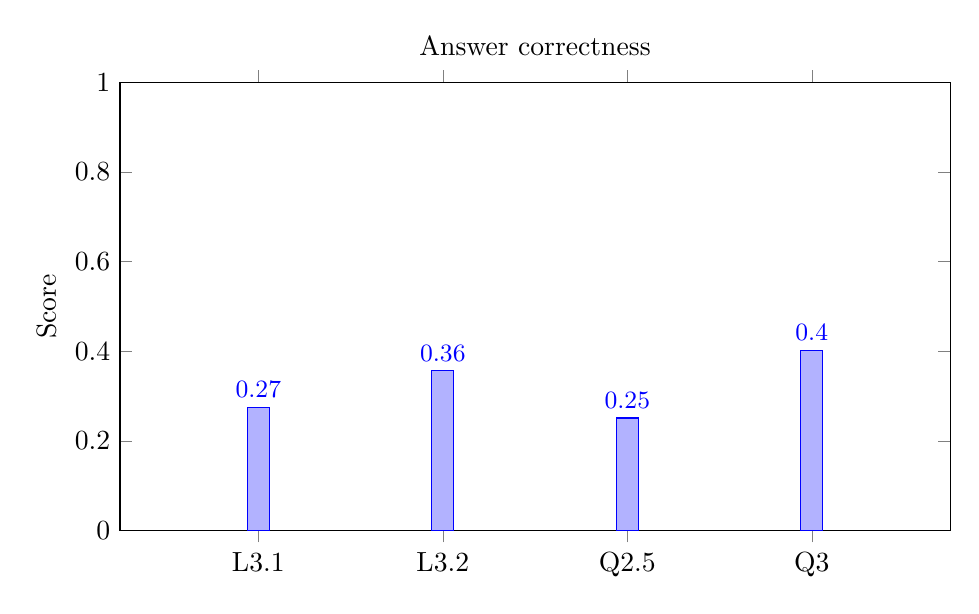
\begin{tikzpicture}
            \begin{axis}[
                ybar,
                ymin=0,
                ymax=1,
                bar width=8pt,
                width=\textwidth,
                height=0.6\textwidth,
                enlarge x limits=0.25,
                ylabel={Score},
                symbolic x coords={L3.1,L3.2,Q2.5,Q3},
                xtick=data,
                nodes near coords,
                nodes near coords align={vertical},
                every node near coord/.append style={font=\small},
                title={Answer correctness}
                ]
                \addplot coordinates {(L3.1,0.274) (L3.2,0.356) (Q2.5,0.251) (Q3,0.402)};
            \end{axis}
        \end{tikzpicture}
    \end{subfigure}
    \hfill
    \begin{subfigure}{0.48\textwidth}
        \centering
        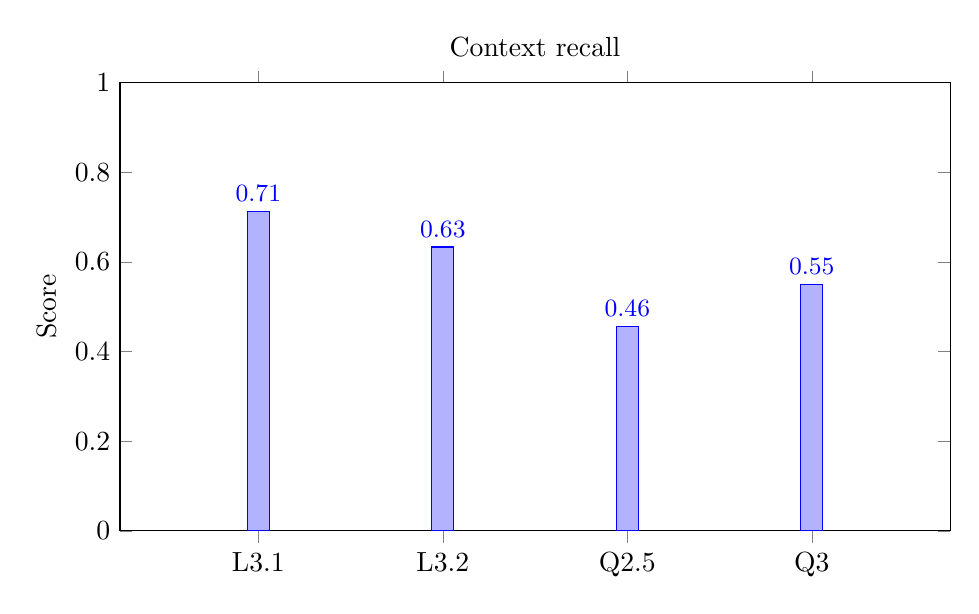
\begin{tikzpicture}
            \begin{axis}[
                ybar,
                ymin=0,
                ymax=1,
                bar width=8pt,
                width=\textwidth,
                height=0.6\textwidth,
                enlarge x limits=0.25,
                ylabel={Score},
                symbolic x coords={L3.1,L3.2,Q2.5,Q3},
                xtick=data,
                nodes near coords,
                nodes near coords align={vertical},
                every node near coord/.append style={font=\small},
                title={Context recall}
                ]
                \addplot coordinates {(L3.1,0.713) (L3.2,0.633) (Q2.5,0.456) (Q3, 0.550)};
            \end{axis}
        \end{tikzpicture}
    \end{subfigure}
    
    \caption{Vergelijking van de prestaties per metric voor alle modellen.}
    \label{fig:vergelijking_metrics}
\end{figure}

Gemiddeld over de vier categorieën scoren de modellen als volgt:

\begin{figure}[H]
    \centering
    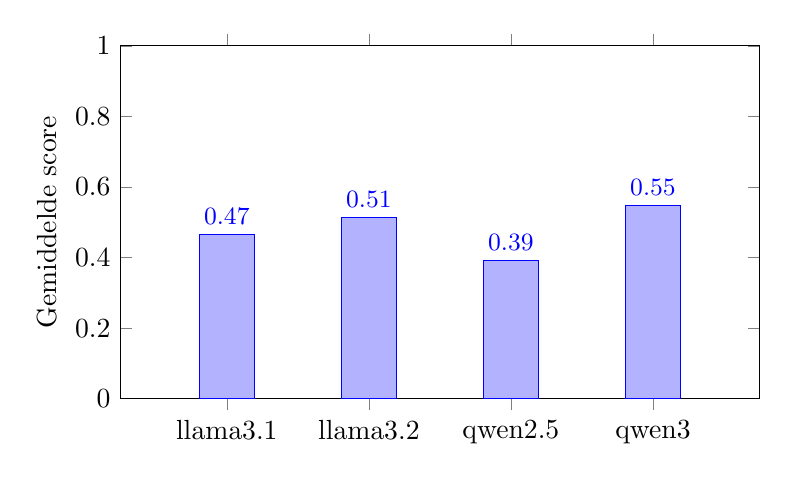
\begin{tikzpicture}
        \begin{axis}[
            ybar,
            ymin=0,
            ymax=1,
            bar width=20pt,
            width=0.8\textwidth,
            height=0.5\textwidth,
            enlarge x limits=0.25,
            ylabel={Gemiddelde score},
            symbolic x coords={llama3.1,llama3.2,qwen2.5,qwen3},
            xtick=data,
            nodes near coords,
            nodes near coords align={vertical},
            every node near coord/.append style={font=\small},
            ]
            \addplot coordinates {(llama3.1,0.466) (llama3.2,0.514) (qwen2.5,0.391) (qwen3,0.548)};
        \end{axis}
    \end{tikzpicture}
    \caption{Gemiddelde score per model.}
    \label{fig:gemiddelde_score_per_model}
\end{figure}

\begin{table}[H]
    \begin{tabular}{|l|c|c|c|c|c|}
        \hline
        \textbf{Model} & \textbf{Faithfulness} & \textbf{Response relevancy} & \textbf{Answer correctness} & \textbf{Context recall} \\
        \hline
        \textbf{llama3.1} & 0.604 & 0.272 & 0.274 & \textbf{0.713} \\
        \textbf{llama3.2} & 0.620 & \textbf{0.445} & 0.356 & 0.633 \\
        \textbf{qwen2.5}  & 0.769 & 0.087 & 0.251 & 0.456 \\
        \textbf{qwen3}    & \textbf{0.880} & 0.358 & \textbf{0.402} & 0.550 \\
        \hline
    \end{tabular}
    \caption{Vergelijking van modelprestaties.}
    \label{tab:modelvergelijking}
\end{table}

\section{Evaluatie 2: Vragen buiten documentatie}

%TODO

\section{Evaluatie 3: Triviale vraagstelling}

Tijdens deze test kreeg ieder model een reeks van vijf triviale vragen voorgelegd. De resultaten van deze test werden verzameld aan de hand van de stacktrace van ieder model, te vinden in bijlage \ref{stacktrace-triviale-vragen}. Op die manier wordt duidelijk welk model direct antwoordt en welk model dat niet doet. Hieronder volgt een overzicht van de verschillende vragen:

\begin{enumerate}
    \item Hallo hoe gaat het?
    \item Hoeveel dagen zitten er in een week?
    \item Wat is 2 + 2?
    \item In welk land ligt Parijs?
    \item Hoeveel minuten zitten er in een uur?
\end{enumerate}

Beide Llama-modellen maakten bij elke vraag onterecht gebruik van de tool. Met andere woorden, zowel het Llama 3.1- als het Llama 3.2-model voerden de flow meerdere keren uit voordat er een antwoord werd gegeven. De Qwen-modellen deden het tegenovergestelde, zij genereerden direct bij elke vraag meteen een antwoord.


